\documentclass{template/openetcs_article}
%\documentclass{article}
%\usepackage[ascii]{inputenc}
%\usepackage[T1]{fontenc}
\usepackage[english]{babel}
\usepackage{amsmath}
\usepackage{amssymb,amsfonts,textcomp}
\usepackage{array}
\usepackage{supertabular}
\usepackage{hhline}
\usepackage{graphicx}
\makeatletter
\newcommand\arraybslash{\let\\\@arraycr}
\makeatother
\setlength\tabcolsep{1mm}
\renewcommand\arraystretch{1.3}
\newcounter{Ilustracin}
\renewcommand\theIlustracin{\arabic{Ilustracin}}
\title{openETCS}

%\setcounter{tocdepth}{3}

\usepackage{hhline}
\usepackage{booktabs}
\usepackage{multirow}
\usepackage{color, colortbl}
\definecolor{myblue}{rgb}{0.6,.6,1}
\definecolor{mydarkblue}{rgb}{0,0,0.5}
\definecolor{mylightblue}{rgb}{0.8,0.8,1}
\usepackage{hyperref}
\hypersetup{colorlinks=true, linkcolor=mydarkblue, urlcolor=mydarkblue}

\usepackage[textwidth=2.7cm,textsize=scriptsize,linecolor=green!40,backgroundcolor=green!40]{todonotes}

\newcounter{mycommentcounter}
\newcommand{\mycomment}[2][]
{
\refstepcounter{mycommentcounter}%
\todo[color={red!100!green!33}]{
\textbf{[\uppercase{#1} \themycommentcounter]:} #2}
}


\usepackage{lipsum,url}
\graphicspath{{./template/}{.}{./images/}}
\begin{document}
\frontmatter
\project{openETCS}

%Please do not change anything above this line
%============================
% The document metadata is defined below

%assign a report number here
\reportnum{OETCS/WP1/D1.3.1}

%define your workpackage here
\wp{Work-Package 1: ``Management''}

%set a title here
\title{Project Quality Assurance Plan - Review Process}

%set a subtitle here
%\subtitle{A template for short document. Adapted from report template.}

%set the date of the report here
\date{\today}

%define a list of authors and their affiliation here

\author{SQS}

\affiliation{Avda. Zugazarte 8,6\\
  48930 Getxo \\
  Vizcaya, España}


% define the coverart
\coverart[width=350pt]{openETCS_EUPL}

%define the type of report
\reporttype{Description of work}




%=============================
%Do not change the next three lines
\maketitle
\tableofcontents
%\listoffiguresandtables
\newpage
%=============================

% The actual document starts below this line
%=============================


%Start here



%\begin{document}


\section*{Document History}

\begin{flushleft}
%\tablefirsthead{\hline Version & Date & Chapters modified & Reason & Name\\}

\tablehead{\hline \rowcolor{myblue} Version & Date & Chapters modified & Reason & Name\\}

\tabletail{}
\tablelasttail{}
\begin{supertabular}{m{1.1cm}m{1.8cm}m{2cm}m{5cm}m{4cm}lp{6cm}|}
\hline
0.0.1 &
09.04.2013 &
All &
First version &
SQS

\end{supertabular}
\end{flushleft}

\newpage

\section[Introduction]{Purpose of the document}
This document presents the whole review process to follow when a document needs revision. It aims to provide a set of guidelines as technical instructions for each review cycle launched that highlights the steps to take.The roles involved in the process are clearly identified as well as their responsibilities and tasks. And finally, the mechanisms needed to achieve the proposed objectives are also included, so the process can be carried out successfully.

\section{Structure of the repository}
 
The review process involves the creation of the following directories inside the structure of each repository. 

\todo{BerndHekele: I propose to document the status of the documents also in the ReadMe of the repository. The following information is of value: Document, review status or review plan. This information can give guidance to the repository}

\todo{BerndHekele: Abbreviation RC is missing and meaning is not clear even though the term is used all over the document}
\begin{flushleft}

\todo{BerndHekele: we need to support also reviews of different nature, e.g., MS-Word, MS-Project, MS-Excel. In this situation I propose to make the PDF file available and make use of the "traditional" review procedure. The decision on this alternative procedure must be part of the review process, i.e., part of the invitation.}

\todo{BerndHekele: a traditional review procedure as used in the section of requirements documents should be the exception, but has to be possible for documents not reasonable in text structures.}

\todo{BerndHekele: it might also be an option to introduce a light-weight review-process for not-critical documents. This process could be based on a slimmed procedure in the issue tracker (like voting or starting an issue on Git. This user guideline should show a little bit like a decision matrix how to select the right procedure.}

\todo{BerndHekele: I propose we also define a section in each document (type) showing the status of the document and the documents history (like your "Document History")}

\begin{tabular}{|m{3cm}|m{11cm}|}
\hline
\rowcolor{myblue}
\multicolumn{2}{|c|}{Structure of the repository} \\\hline
\rowcolor{lightgray}
Name &
Content 
\\\hline
Final documents &
Pdf final documents validated after a RC is closed by the responsible of the document.\\\hline
Review Documents &
\begin{itemize}
\item A control sheet: With the basic information of the review cycle.
\item The review document: In Tex format with all its history of changes.
\end{itemize}\\\hline
\end{tabular}
\end{flushleft}

\section{Roles}


This section describes  the roles of the participants in the review process of the documentation:

\begin{flushleft}

\begin{tabular}{|m{3cm}|m{11cm}|}
\hline
\rowcolor{myblue}
\multicolumn{2}{|c|}{Roles} \\\hline
\rowcolor{lightgray}
Role &
competencies \\\hline
RC manager / Owner of the document &
\begin{itemize}
\item Launch the Review Process
\begin{itemize}
\item RC Request.
\begin{itemize}
\item Justify the new RC. ({\it TI.6.3.1 New RC Request})
\end{itemize}
\item Open a review cycle for a document. To do this, create a git new branch ({\it TI.6.1.1. New RC branch}) 
\item Open a new issue for the new RC linked to the document and the review. Only the owner of the document can close the issue and he/she also be in charge of conducting the discussions and comments below the issue.  ({\it TI.6.1.2. Open issue})
\item Create the Control Sheet with the basic information related to the tasks to be done during the complete new cycle. ({\it TI.6.1.3. Complete the Control Sheet})
\item BerndHekele: In each review cycle the manger has to decide who is mandatory contributor in the review. Mandatory Contributors have to be invited (per mail or phone) personally and need to confirm participation in the requested time period (effort is covered).

\item BerndHekele: We should foresee the option of a personal meeting or a \"goto-meeting\" when inviting to intensive documents. This has to be decided at the start of the RC and may be requested later if intensive discussions are ongoing during the review.

\end{itemize}
\item Control Review Process
\begin{itemize}
\item Supervision of the work done. ({\it TI.6.1.4. Supervision of the Review Process})
\end{itemize}
\item Accept/Reject
\begin{itemize}
\item Use todonotes tool to add, verify and reject comments in the document being reviewed. ({\it TI.6.3.2 Add notes using todonotes})
\item Make changes to the document.
\item BerndHekele: after updating the document the owner shall distribute the document for a final confirmation of the changes. Typically, this process shall only allow a few days for final confirmation. This step is essential if criticial issues have been detected or discussed during the review.

\end{itemize}
\item Closing
\begin{itemize}
\item Send the notification of closing. ({\it TI.6.1.6. RC Issue closing})
\item Merge the associated RC branch into the repository master branch. ({\it TI.6.1.7. RC Branch merging})
\item Generate an established version of the document in PDF format when the review cycle is finished and store it in the directory of Final documents. ({\it TI.6.1.8. Pdf delivery})
\end{itemize}
\end{itemize}
\\\\\hline
\end{tabular}
\end{flushleft}
\todo{BerndHekele: the valid options of the todonotes tool are not documented in the proposed location}

\begin{flushleft}

\begin{tabular}{|m{3cm}|m{11cm}|}
\hline
\rowcolor{myblue}
\multicolumn{2}{|c|}{Roles} \\\hline
\rowcolor{lightgray}
Role &
competencies 
\\\hline
Reviewer &
\begin{itemize}
\item RC Request.
\begin{itemize}
\item Justify the RC Request and explain the interest in collaborating. ({\it TI.6.3.1 New RC Request})
\end{itemize}
\item Review Work
\begin{itemize}
\item Prepare the working environment: To change the document, the committer has to clone the repository in local, create a branch and associate to the repository on gitHub ({\it TI.6.2.1. Review environment setup}).
\item Be aware of how to perform the review work ({\it TI.6.2.2 Review work})
\item Make comments, suggestions or improvement proposals with the todonotes package installed for the LaTeX editing tool. ({\it TI.6.3.2 Add notes using todonotes})
\item Comment in the issue thread in the git repository. ({\it TI.6.3.3 Add comments in a RC issue})
\end{itemize}
\end{itemize}
\\\hline
\end{tabular}
\end{flushleft}


\section{Tools}

\begin{flushleft}

\begin{tabular}{|m{3cm}|m{11cm}|}
\hline
\rowcolor{myblue}
\multicolumn{2}{|c|}{Tools} \\\hline
GIT &
\begin{itemize}
\item GitHub: A web-based hosting service for projects that use Git revision control system.
\item SmartGit: A graphical front-end for Git distributed version control systems. 
\end{itemize}\\\hline
Pdf documents &
\begin{itemize}
\item Adobe Acrobat Reader: Software package that allows to view, navigate and print pdf files.
\item Diffpdf: Open source application that compares different PDF files for discrepancies. 
\item BerndHekele: PDF Creator: Software for creating pdf files. Works like a printer on your PC.

\end{itemize}\\\hline
TeX documents &
\begin{itemize}
\item MiKTeX : Provides the tools necessary to prepare documents using de TeX/LaTeX mark up language.
\item GhostScript. 
\item GhostView.
\item TexMaker.
\item Todonotes package.
\item Adobe Acrobat Reader: Software package that allows to view, navigate and print pdf files.
\item BerndHekele: I would like to see in addition a tool to compare files (outside of SmartGit). I have seen no open source solution so far. But, maybe someone else knows a good solution.

\end{itemize}\\\hline
\end{tabular}
\end{flushleft}

\section{Review Process Overview}

\todo{BerndHekele: I see this document as a good basis for textual documents in the process. However, we also need to decide how we live the process for other documents like Code of formal specifications. We need to be prepared for those kind of documents before actual reviews start. We do not have to much time.}

This subject is concerned with the validation and verification of the documentation generated within the OpenETCS project.  The process shall aim to confirm that what has been produced is correct and meets the expectations of the committers as well as improving the quality of the document and its reliability; it also ensures the technical approach is appropriate before releasing the related documentation.

The Review Process refers to documents that are prone to be under review consideration because the authors have delivered its first release, some sections have been included or any committee has considered an improvement. 

This whole process is independent from the habitual work done in the repositories; so, whereas the OpenETCS members work as usually do in the master branch, the new Review Cycle shall be attached to a specific repository branch (previously created by the document owner). Then any change, comment, suggestion or improvement to do to the identified document under review, shall be done inside this RC branch and in the correspondent ‘review\_documents’ directory inside the OpenETCS structure. 

In this way, the day to day work with regard to the master branch shall not be affected by the work being done in the review context; the whole review cycle for a specific document shall be linked to a specific branch of the repository. 
This is the key of the process because with this mechanism there shall be no dependencies between the ordinary work done in the project and the different review cycles launched for different documents at different times.

During their lifetime, these documents shall be involved at least in one complete Review Cycle, but it there will be as many review cycles as considered necessary. The different Review Cycles linked to each document shall be numbered and associated to their branches.   

A Review Cycle will help the project to better meet its strategic goals and objectives, so the correctness of the deliverables is ensured and they cover their intended purpose.

In this context the review will help to:
\begin{itemize}
\item Identify deficiencies that shall be fixed. Reviewing a document in a structured way will identify problems or faults with that product. Applying a methodology for reviews shall take advantage of the expertise and knowledge of the committers involved with a greater proportion of improvements and defects found.
\item Ensure the coherence, correct use of language and appropriate structure.
\item Collect recommendations and improvements suggested by the committers so the document is enriched with specific experiences and multiple points of view and technical perspectives.
\end{itemize}

The key aspects of the review process include the following:

\begin{itemize}
\item \underline{Each review need for a document shall be translated into the creation of a new review cycle}
\begin{itemize}
\item A RC for a document starts when a need or objective to be fulfilled is identified.
\item Such proposal can be done by the owner of the document or by any committer that can justify the need for a new cycle. 
\item When a proposal is submitted by a person who is not the owner of the document, the review proposal shall be accepted by the owner of the document and the process shall begin.
\item BerndHekele: review cycles are timeboxed. When starting the cycle the review plan and the end date for the review need to be confirmed.
 
\end{itemize}
\item \underline{The owner of the document shall be the RC manager}
\begin{itemize}
\item The owner of the document to be reviewed shall be the responsible for addressing and conducting the review during the expected time of the cycle. 
\item He/she shall be aware of the tasks that are their responsibility, so the review is under control, the steps defined in the technical procedure are correctly followed and known, and it can be conducted with minor incidents. 
\end{itemize}

\item \underline{Close collaboration between the RC manager and the reviewers}
\begin{itemize}
\item The participants in the review shall be guided by the RC manager in the whole process so the optimum level of collaboration and integration is reached. 
\item Any conflict detected when uploading the review in the repository, question or problem found by any reviewer at any moment shall be communicated via the opened issue thread, and the RC manager shall be responsible for providing the appropriate support.
\end{itemize}

\item \underline{The documentation needed for performing the review shall be always accessible in an easy way.}

\begin{itemize}
\item Once the issue announcing the new Review Cycle has been published, the participants can have access to the needed information and documentation in the review\_documents directory.
\item Each Review Cycle identified for a document shall have a detailed Control Sheet with all the information needed, the tasks assigned when there is not an open a general review, the objectives to meet, deadlines, etc. support.
\end{itemize}

\item \underline{The review shall be done locally by the reviewers}
\begin{itemize}
\item Using the Smartgit tool the reviewers shall ensure that they have switched their work context to the required RC branch and then synchronize the contents so they have the last committed version of the review\_directory.
\item The reviewers shall work in the cloned repository that contains the document under review locally 
\item They shall use the todonotes package installed for the LaTeX editing tool to include comments and suggestions into the document under review
\end{itemize}

\item \underline{The reviewer is responsible for uploading the changes to the remote branch}
\begin{itemize}
\item Once the work is done, the reviewer shall ensure he/she has the last committed version of the document under review before pushing the changes into the correspondent git repository. 
\item The conflicts that can appear due to simultaneous work in the same document shall be resolved before merging the changes into the document under review. 
\item When the review is uploaded the reviewer shall notify the actualization by sending a message in the opened issue thread.
\item The reviewer shall wait for the RC manager to approve or reject the proposed changes.
\end{itemize}

\item \underline{The RC manager shall decide when the Review Process is closed}
\begin{itemize}
\item The reviewer shall receive a notification by e-mail, and publicly in the opened related issue, once the RC manager has checked the proposed review. 
\item The reviewers shall continue working with the document in case there are still pending issues.
\item When there are no more pending issues, neither comments nor suggestions to be done, the review process is finished. Then, the RC manager shall be the responsible for 
\begin{itemize}
\item closing the corresponding issue in the repository, 
\item sending the notification of closing, 
\item merging the associated RC branch into the repository master branch, 
\item generating an established new version of the document 
\item and uploading it into the Final documents directory in the repository.
\end{itemize}
\end{itemize}

\end{itemize}

There can be in the git repository different intermediate versions in pdf of the document under review in the review\_documents directory. However, this pdf document can be used only as a quick reference of the progress of the review, and it cannot be taken as a final document. 

It is important to have in mind that the document under review, once it has been verified and approved by the RC manager, shall be available in the Final documents directory.

In the Final documents directory of each WP inside the structure of the OpenETCS project there shall be always a readable version for anyone in the project. 

When comparisons between correlative stable versions of a document need to be done, the diffPDF tool cab be used to find the differences between them.


\section{Technical Instructions}

In this section the whole Review process is explained step by step using technical instructions, so all the participants involved in the process are aware of the mechanisms they shall implement to work and achieve the expected objectives. 

The sequence of activities or course of action that must be followed by the reviewers as well as the RC manager is explained below. 


\subsection{Technical Instructions for the RC Manager}

This section includes the Technical Instructions the RC manager shall be aware of.

\subsubsection{New RC branch}

\begin{flushleft}
\tablefirsthead{}
\tablehead{}
\tabletail{}
\tablelasttail{}
\begin{supertabular}{|m{2cm}|m{13cm}|}
\hline
\rowcolor{myblue}
TI & 
TI.6.1.1. New RC branch
\\\hline
Roles &
RC manager
\\\hline
Description &
Any changes made to the document under review to include comments, recommendations or additional sections shall be made in a RC branch context. The RC manager shall create the branch and makes it available for the reviewers.
\\\hline
Steps &
\begin{itemize}
\item Steps to create the branch locally are:
\begin{enumerate}
   \item Open Smartgit
   \item Branch menu, add branch and give a new name following this nomenclature: 
   \begin{itemize}
   \item {\it RC\_<name of the document to be reviewed>\_<number of review>}. 
   \end{itemize}
   \item Push {\it add branch \& switch}. With these steps the branch is created as a local branch.
\end{enumerate}
\item Integrate the branch into the git repository
\begin{enumerate}
	\item Go to the toolbar and press {\it Push}, accept then the messages. 
	\item The new branch appears in the Smartgit Branches view, below the origin tag. 
	\item Confirm that the local branch is linked to the remote git branch: in the local one the {\it set tracked branch shall} have been done and it shall address to the RC branch already created in the git repository
\end{enumerate}
\end{itemize}
\\\hline
\end{supertabular}
\end{flushleft}

\begin{figure}
\centering
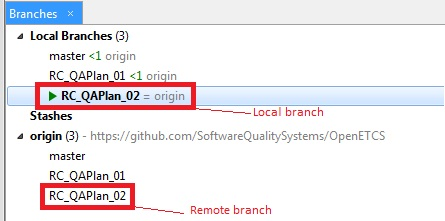
\includegraphics {./figures/Branches.JPG}
\caption{Branches tree in {\it Smartgit}}
\end{figure}


\subsubsection{Open a New issue in the repository}

\begin{flushleft}
\tablefirsthead{}
\tablehead{}
\tabletail{}
\tablelasttail{}
\begin{supertabular}{|m{2cm}|m{13cm}|}
\hline
\rowcolor{myblue}
TI & 
TI.6.1.2. Open issue
\\\hline
Roles &
RC manager
\\\hline
Description &
A new issue shall be opened to contain the discussions, comments and notifications related to a specific RC for a document.
\\\hline
Steps &
\begin{itemize}
\item Create a new issue in the repository that contains the document under review. 
\begin{enumerate}
   \item Open Github and go to the correspondent repository
   \item Select the {\it Issues section}
   \item Push the {\it New issue} button
   \item Add a descriptive title indicating the name of the new RC and the document under review
   \item Add a significant description about the causes that have motivated the new RC and summarizes the objectives of the review. In case there are specific reviewers involved, provide their names.
   	\item Push {\it Submit new issue}
\end{enumerate}
\item Notify the opening of the issue to the reviewers involved when there are specific names involved
\begin{enumerate}
	\item Send an e-mail to all the reviewers involved when the RC is limited to a group of known people 
\end{enumerate}
\end{itemize}
\\\hline
\end{supertabular}
\end{flushleft}

\begin{figure}
\centering
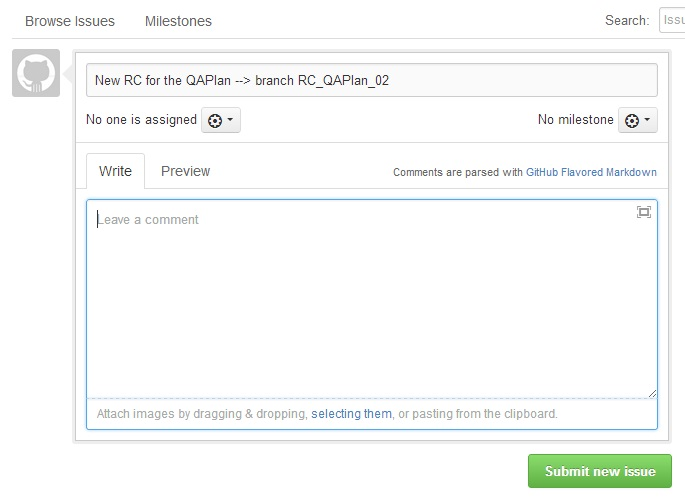
\includegraphics [width=\textwidth]{./figures/NewIssue.JPG}
\caption{New issue in {\it Github}}
\end{figure}

\subsubsection{Complete the Control Sheet}

\begin{flushleft}
\tablefirsthead{}
\tablehead{}
\tabletail{}
\tablelasttail{}
\begin{supertabular}{|m{2cm}|m{13cm}|}
\hline
\rowcolor{myblue}
TI & 
TI.6.1.3. Complete the Control Sheet
\\\hline
Roles &
RC manager
\\\hline
Description &
A Control Sheet shall be prepared so all the basic and pertinent information of the review is available to all the reviewers involved. The RC manager shall indicate as much information as possible about the deadlines, the objectives to be met, the tasks assigned to specific reviewers when it is a limited review, and any information he/she considers relevant to accomplish the Review Process
\\\hline
Steps &
\begin{itemize}
\item Take the Control Sheet Template as reference. It contains a set of columns that shall be completed
\begin{enumerate}
\item The sheet shall be available in the Review Process directory available in the {\it governance} repository
\item The responsible of the Review Cycle: the owner of the document shall be the responsible so their name is indicated in the sheet
\item Name of the document to be reviewed
\item Needs, objectives or improvements identified that justify the new review cycle.
\item The branch created for the review, so the reviewers can change their contexts to the specific branch and work from this point on with that. For any other works the reviewers are doing, they shall be aware that they must leave the change before uploading any new version.
\item Participants involved in the process: the RC could include any committer that wants to participate or could be addressed to specific committers. The specific case is explained in detail in the sheet. Whenever specific participants are identified the specific tasks for each of them are clearly proposed.
\item Starting date and deadline.
\end{enumerate}
\item Add additional information whenever it is necessary
\item Put the Control Sheet inside the {\it Reviews directory} available for the document under review
\end{itemize}
\\\hline
\end{supertabular}
\end{flushleft}

\begin{figure}
\centering
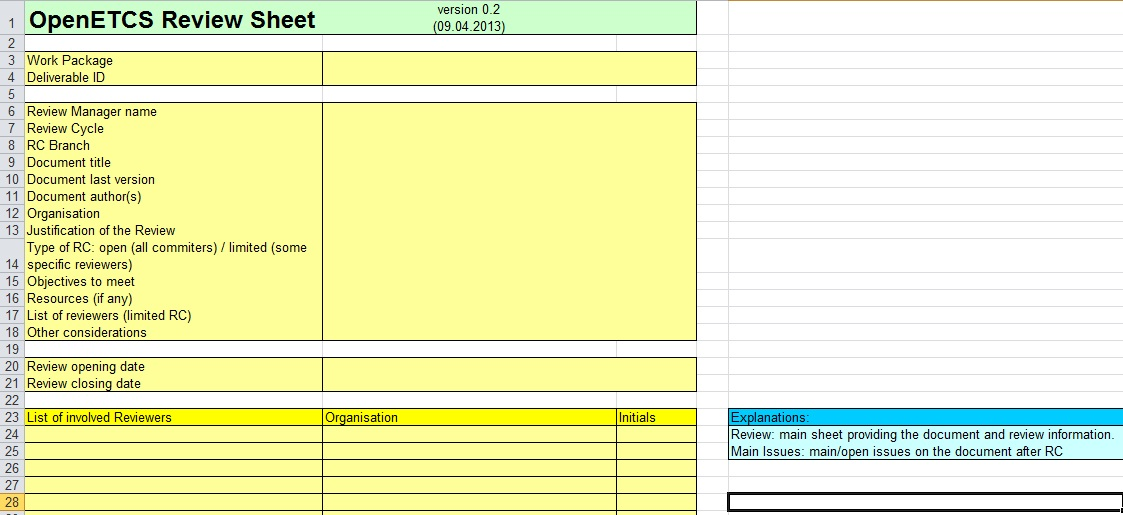
\includegraphics [width=\textwidth]{./figures/ControlSheet.JPG}
\caption{Template of the Control Sheet}
\end{figure}

\subsubsection{Supervision of the Review Process}

\begin{flushleft}
\tablefirsthead{}
\tablehead{}
\tabletail{}
\tablelasttail{}
\begin{supertabular}{|m{2cm}|m{13cm}|}
\hline
\rowcolor{myblue}
TI & 
TI.6.1.4. Supervision of the Review Process
\\\hline
Roles &
RC manager
\\\hline
Description &
The RC Manager shall be responsible for assessing the progress done in the RC
\\\hline
Steps &
\begin{itemize}
\item The RC manager shall wait for the reviewers to answer, so they confirm the pending issues have been fixed or they have more suggestions to do.
\item The iterative work done in a RC shall finish once the RC manager and reviewers have reached a common agreement about the state of the document, and no more issues are pending. \item When this happens, the RC manager shall clean the document, deleting all the comments, confirmations and notes inserted into the document, so a final editable version is obtained.
\end{itemize}
\\\hline
\end{supertabular}
\end{flushleft}

\subsubsection{Approval/rejection of comments}

\begin{flushleft}
\tablefirsthead{}
\tablehead{}
\tabletail{}
\tablelasttail{}
\begin{supertabular}{|m{2cm}|m{13cm}|}
\hline
\rowcolor{myblue}
TI & 
TI.6.1.5. Approval/rejection of comments
\\\hline
Roles &
RC manager
\\\hline
Description &
The RC manager shall study each proposal, recommendation or comment that appears in the document under review and decide how to implement the proposed changes in case he/she estimates it is appropriate to be included in the document.  
\\\hline
Steps &
\begin{itemize}
\item When a reviewer notifies in the RC issue thread that some changes have been uploaded using the corresponding RC branch, the RC manager synchronizes their repository to obtain the last commit made for the document with the {\it SmartGit} tool.
\item He/she reads carefully any annotation that appears in the document and decides whether he/she shall implement that comments or not.
\item For each annotation the RC manager finds in the document, he/she shall provide a written confirmation about what is their decision about the subject. 
\begin{enumerate}
\item Use the {\it todonotes} to confirm/reject proposals made by the Reviewers ({\it TI.6.3.2 Add notes using todonotes}) 
\item The RC manager shall adds a comment confirming or rejecting it. A justification for that decision shall be included.
\item When the suggestion is accepted:
\begin{enumerate}
\item Assess whether the recommendation made implies writing new paragraphs, sections, adding new figures, etc. and modify the document accordingly. 
\item Highlight the new text or the modified text with {\it todonotes} using the {\it inline} option.
\end{enumerate}
\end{enumerate}
\item The RC manager commits the changes made in the document and push them into the RC branch so the reviewers can have access to the changes, confirmations and rejections made by the RC manager.
\item The RC manager adds a message to the RC issue thread so everyone can be informed about the commit recently done. 
\end{itemize}
\\\hline
\end{supertabular}
\end{flushleft}

\begin{figure}
\centering
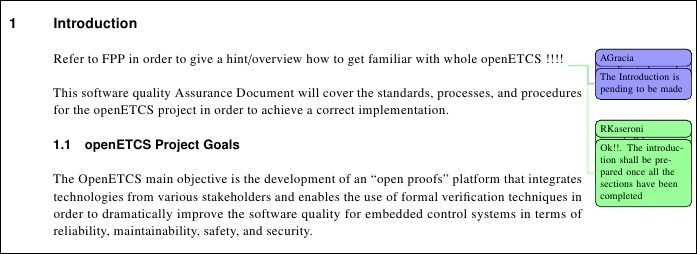
\includegraphics [width=\textwidth]{./figures/CommentConfirmation.JPG}
\caption{New issue in {\it Github}}
\end{figure}

\subsubsection{RC Issue closing}

\begin{flushleft}
\tablefirsthead{}
\tablehead{}
\tabletail{}
\tablelasttail{}
\begin{supertabular}{|m{2cm}|m{13cm}|}
\hline
\rowcolor{myblue}
TI & 
TI.6.1.6. RC Issue closing
\\\hline
Roles &
RC manager
\\\hline
Description &
The RC manager shall be the responsible for closing the current Review Cycle after verifying and confirming all the changes done. The first task to be done is to notify the closing and highlight the results obtained.
\\\hline
Steps &
\begin{itemize}
\item Add a Comment in the issue thread to indicate that the RC has finished
\begin{enumerate}
\item Follow the indications provided in the {\it TI.6.3.3 Add comments in a RC issue} to add a comment
\item Provide a brief summary of the RC:
\begin{enumerate}
\item Indicate the way the objectives have been met 
\item Are there pending objectives?. Indicate the reason for closing the RC before all the objectives have been met.
\item Identify the key aspects of the review
\item Highlight the results obtained
\item Identify improvements for a future Review Cycle for the document under review
\end{enumerate}
\end{enumerate}
\item Close the RC issue thread pushing the {\it Close} button in {\it GitHub}.
\item Notify the closing of the RC when the review process has been carried out by limited Reviewers. The notification shall be made by e-mail.
\end{itemize}
\\\hline
\end{supertabular}
\end{flushleft}

\subsubsection{RC Branch merging}

\begin{flushleft}
\tablefirsthead{}
\tablehead{}
\tabletail{}
\tablelasttail{}
\begin{supertabular}{|m{2cm}|m{13cm}|}
\hline
\rowcolor{myblue}
TI & 
TI.6.1.7. RC Branch merging
\\\hline
Roles &
RC manager
\\\hline
Description &
Merging the {\it RC Branch} to the {\it Master branch} implies incorporating the changes made in a document to the main branch of the repository. In this way, the new release of the editable document is available in the master branch.
\\\hline
Steps &
\begin{itemize}
\item Merge the branches 
\begin{enumerate}
\item Switch to the {\it master branch}, so that the working tree will be the master branch from this moment on
\item With the RC branch selected the RC Manager shall do a click on right button and select {\it merge to working tree}.
\end{enumerate}
\item Confirm the update
\begin{enumerate}
\item Make {\it push} to the repository and the merge shall be done.
\item Make {\it synchronize} so all the changes made are reflected remotely and locally.
\end{enumerate}
\end{itemize}
\\\hline
\end{supertabular}
\end{flushleft}

\subsubsection{Pdf Delivery}

\begin{flushleft}
\tablefirsthead{}
\tablehead{}
\tabletail{}
\tablelasttail{}
\begin{supertabular}{|m{2cm}|m{13cm}|}
\hline
\rowcolor{myblue}
TI & 
TI.6.1.8. Pdf Delivery
\\\hline
Roles &
RC manager
\\\hline
Description &
The RC manager shall deliver the document under review (once the complete RC has finished) in a only-readable format. This versioned, stable and verified release of the document shall be accessible publicly by everyone with the certainty that it is a confirmed work.
\\\hline
Steps &
\begin{itemize}
\item Preparation of the pdf
\begin{enumerate}
\item The RC manager shall compile the document under review in its editable version (LaTex) and obtain a pdf non-editable document.
\item The new document shall be put in the appropriate repository, inside the {\it Final documents} directory.
\end{enumerate}
\item Notification of the update
\begin{enumerate}
\item A notification of the update shall be done publicly, posting a new Issue in the repository that shall be labelled as {\it enhancement}. 
\end{enumerate}
\end{itemize}
\\\hline
\end{supertabular}
\end{flushleft}

\subsection{Technical Instructions for the Reviewers}

This section includes the Technical Instructions the Reviewers shall be aware of.

\subsubsection{Review Environment setup}

\begin{flushleft}
\tablefirsthead{}
\tablehead{}
\tabletail{}
\tablelasttail{}
\begin{supertabular}{|m{2cm}|m{13cm}|}
\hline
\rowcolor{myblue}
TI & 
TI.6.2.1. Review environment setup
\\\hline
Roles &
RC manager
\\\hline
Description &
Each Reviewer shall prepare the working environment locally and ensure it is ready before starting with the review tasks.
\\\hline
Steps &
\begin{itemize}
\item Setup using {\it Smartgit} tool
\begin{enumerate}
\item Clone the repository with the {\it Project --> Clone} option.
\item Go to the {\it Branch} menu, select {\it Add branch} and give a name. Then, the branch is created as a local branch.
\item Link the local branch to the remote git branch, to do that, select {\it Set tracked branch} in the context menu of the local branch. The local environment is then ready for working in the Review Process
\end{enumerate}
\item Update the environment
\begin{itemize}
\item It is essential to work in the last release of the document under review, so minimal conflicts appear in the future when uploading the changes. To be sure about this, a pull request shall be done to the repository before editing the document.
\begin{itemize}
\item Select the {\it Pull} option on the toolbar
\end{itemize}
\end{itemize}
\end{itemize}
\\\hline
\end{supertabular}
\end{flushleft}

\subsubsection{Review work}

\begin{flushleft}
\tablefirsthead{}
\tablehead{}
\tabletail{}
\tablelasttail{}
\begin{supertabular}{|m{2cm}|m{13cm}|}
\hline
\rowcolor{myblue}
TI & 
TI.6.2.2 Review work
\\\hline
Roles &
Reviewers
\\\hline
Description &
The Reviewer shall perform the review in the expected time and conditions and the starting point shall be provided by the Control Sheet prepared by the RC manager and the work. The work of a reviewer shall finished when the RC owner confirms the closing of the RC.
\\\hline
Steps &
\begin{itemize}
\item The Reviewer shall:
\begin{enumerate}
\item Make comments, suggestions or improvement proposals with the {\it todonotes} (See {\it TI.6.3.2 Add notes using todonotes}).
\item Add comments in the RC issue thread when it applies (See {\it TI.6.3.3 Add comments in a RC issue}).
\item Make changes in the document. Each insertion shall be highlighted indicating the initials of the Reviewer. The review process shall be done by different people and what comments have been written by whom shall be known.
\end{enumerate}
\item The reviewer shall integrate the changes to the document that is hosted in the remote repository in GitHub. 
\item To do that, click on the {\it Push} button in the SmartGit tool. When pushing different situations can happen:
\begin{itemize}
\item There are no conflicts with the original repository .
\begin{enumerate}
\item The changes shall be included.
\end{enumerate}
\end{itemize}
\begin{itemize}
\item There are one or more conflicts.
\begin{enumerate}
\item Click on the {\it Pull} button so the last version is loaded. 
\item Open the {\it Conflict Solver} Window to compare the committed version in the {\it Github} and the local version. 
\item The conflict shall be solved in the following way.
\begin{enumerate}
\item The reviewer shall indicate that the version stored in the remote repository is the correct one. The changes in case of conflict are not included. 
\item The Reviewer will {\it Push} the changes that do not have any conflict and add a notification in the document about that. 
\item After finishing the {\it pushing}, he/she shall perform a {\it pulling} to obtain the integrated and last committed version; then he/she shall add a note using {\it todonotes} tool in the section where the conflicts were; he/she shall explain the problem found. 
\end{enumerate}
\item Have in mind that after {\it pushing/pulling} the document the changes in conflict made by the Reviewer shall be lost. Anytime a conflict appears, the reviewer shall prepare a copy of the suggestions or modifications made by him/her.
\item He/she also adds a comment in the RC issue thread exposing that problem in the document and requesting a solution.
\item The RC Manager shall take part in the discussion and propose a solution. The Reviewer can put in the document again the suggestions in conflict stored locally if the RC manager requires that.
\end{enumerate}
\end{itemize}
\end{itemize}
\\\\\hline
Steps &
\begin{itemize}
\item In any case, the reviewer shall inform about the progress of their work posting a message in the RC issue thread. From this point, the reviewer shall wait for the RC manager to read the proposed review and provide comments. (See {\it TI.6.3.3 Add comments in a RC issue}).
\end{itemize}
\\\hline
\end{supertabular}
\end{flushleft}

\begin{figure}
\centering
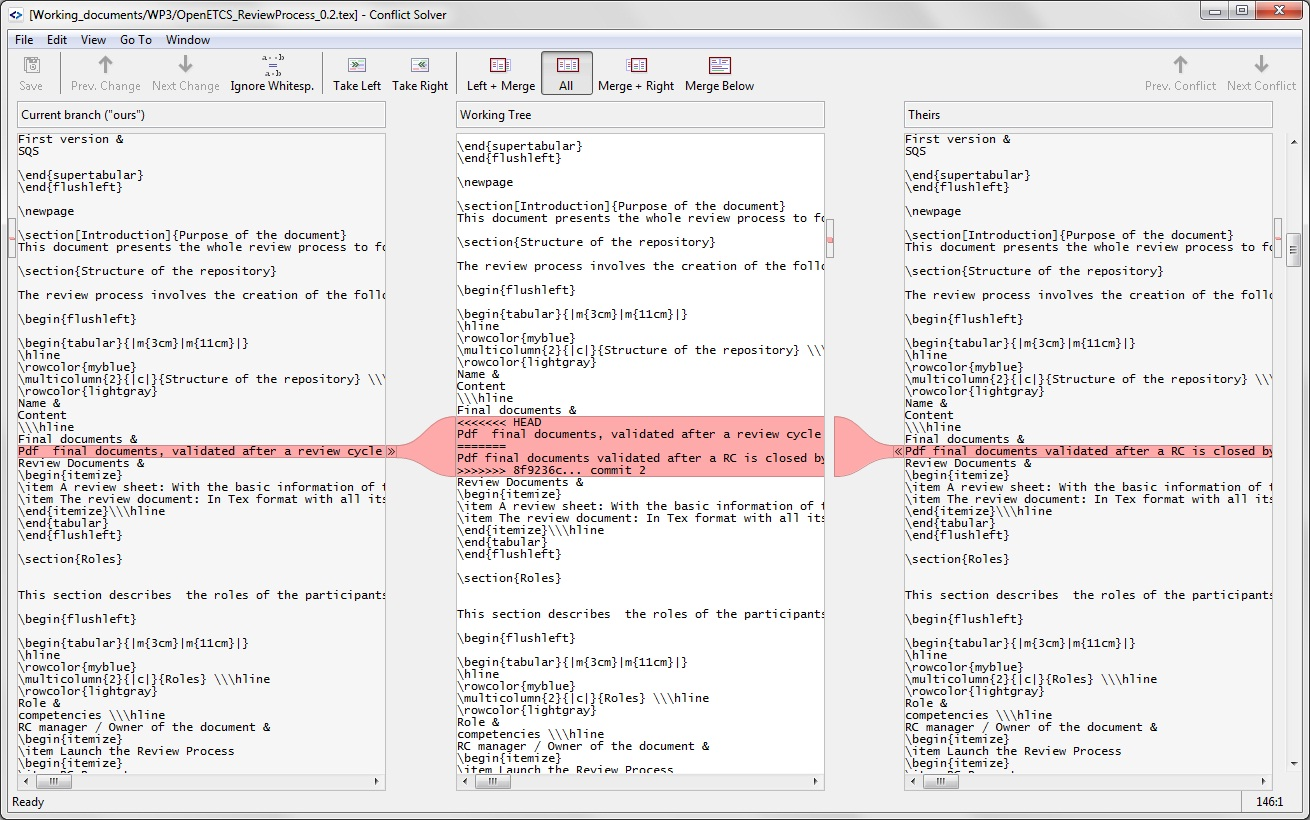
\includegraphics[width=\textwidth]{./figures/ConflictSolverWindow.JPG}
\caption{Conflict Solver Window}
\end{figure}

\subsection{Technical Instructions for any Role}
This section includes any Technical Instruction that shall be followed by the RC manager or Reviewers at different phases of the Review Process

\subsubsection{New RC request}

\begin{flushleft}
\tablefirsthead{}
\tablehead{}
\tabletail{}
\tablelasttail{}
\begin{supertabular}{|m{2cm}|m{13cm}|}
\hline
\rowcolor{myblue}
TI & 
TI.6.3.1 New, RC request
\\\hline
Roles &
RC manager
Any committer
\\\hline
Description &
Any person belonging to the OpenETCS project can prepare a review proposal and make a request. 
\\\hline
Steps &
\begin{itemize}
\item The proposer is the owner of the document
\begin{itemize}
\item A member of the project has finished a document and proposes a general review of contents and structure
\item The owner of a document is interested in receiving several suggestions or improvement recommendations by specific experts. 
\begin{enumerate}
\item He/she needs no confirmation for beginning the review. 
\item He/she is responsible for starting the process and takes charge of the preparation of the working environment. 
\end{enumerate}
\end{itemize}
\item The proposer is not the owner of the document
\begin{itemize}
\item The person interested in opening a new review cycle posts a new issue in the repository. 
\begin{enumerate}
\item Appropriate and complete information about the review proposal is required. It shall be justified.
\item The proposal could include suggestions of people who can play the role of Reviewers considering the technical difficulty and the expertise of them.
\end{enumerate}
\item The issue shall be answered by the owner of the document after analyzing the request. 
\begin{itemize}
\item The request is accepted: the owner of the document shall be the RC manager and he/she shall be in charge of opening the RC.
\item The request is rejected: the owner of the document shall provide the reasons that have motivated him/her to denied the proposal. 
\end{itemize}
\end{itemize}
\end{itemize}
\\\hline
\end{supertabular}
\end{flushleft}

\subsubsection{Add notes using todonotes}

\begin{flushleft}
\tablefirsthead{}
\tablehead{}
\tabletail{}
\tablelasttail{}
\begin{supertabular}{|m{2cm}|m{13cm}|}
\hline
\rowcolor{myblue}
TI & 
TI.6.3.2 Add notes using todonotes
\\\hline
Roles &
RC manager, Reviewers
\\\hline
Description &
The package todonotes must be installed locally to make comments in the document under review. 
\\\hline
Steps &
\begin{itemize}
\item Verify the installation of the todonotes package locally. In case the package is not installed, follow these steps:
\begin{enumerate}
\item Got to the {\it MixTex} tool directory, select {\it Maintenance (Admin)} and click on {\it Package Manager (Admin)}.
\item Look for the {\it todonotes} package using the filtering option.
\item Select the package after the search is done and install.
\end{enumerate}
\item Be used to the most common commands available in the package.
\begin{enumerate}
\item Go to the {\it governance} repository in the Github and look for the {\it Reviews Process} folder. There you can find a {\it todonotes} document that explains all the commands that can be used during the reviewing.
\end{enumerate}
\item Identify always any comment done with your initials.
\begin{enumerate} 
\item The initials of the person who inserts a comment into the document shall be the the first letter of the name plus the surname.
\end{enumerate}
\item Use different colours in the document for different meanings 
\begin{enumerate}
\item {\it Red}: indicate in a comment what paragraph, section or line the reviewer propose to delete. This color shall be used also by the RC manager when he/she confirms the suggestion done by a reviewer has been rejected.
\item {\it Green}: the suggestion made by a reviewer has been approved and the RC manager adds a comment with this color.
\item {\it Orange}: the comment refers to any conflict found between commits done by different reviewers.
\item {\it Blue}: any general comment done by the participants in the review. 
\end{enumerate} 
\end{itemize}

\\\hline
\end{supertabular}
\end{flushleft}

\subsubsection{Add comments in a RC issue}

\begin{flushleft}
\tablefirsthead{}
\tablehead{}
\tabletail{}
\tablelasttail{}
\begin{supertabular}{|m{2cm}|m{13cm}|}
\hline
\rowcolor{myblue}
TI & 
TI.6.3.3 Add comments in a RC issue
\\\hline
Roles &
RC manager, Reviewers
\\\hline
Description &
The issue opened by the RC manager at the beginning of the RC shall be used whenever a notification shall be done, conflict reported or questions asked. The collaborative work shall aim to get a dynamic approach when the discussions are fluid, with quick answers and sharing of information.
\\\hline
Steps &
\begin{itemize}
\item Go to the repository where the document under review is located.
\item Select the issue that has the RC you are working on.
\item The comments posted shall be descriptive enough so any reader can understand the message. 
\begin{enumerate}
\item Identified yourself clearly, providing your name and role in the project.
\item When required, include diagrams, figures, partial texts or specific data that help to understand the problematic found.
\end{enumerate}
\item Do not edit any comment done. It is a better option to rewrite it with the additions you proposed than editing and make the changes directly. In this way, it is assured that everyone reads the new message because in the other case, the change/addition can be missed.
\item Push the {\it Comment} button to post the message.
\end{itemize}

\\\hline
\end{supertabular}
\end{flushleft}

\end{document}
